\documentclass{article}
\usepackage{amsmath}
\usepackage{tikz}
\usetikzlibrary{matrix}

\begin{document}

\begin{equation}
\boldsymbol{J} \quad = \quad 
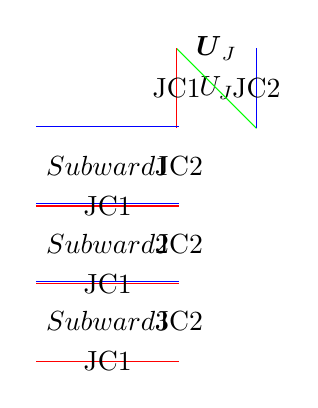
\begin{tikzpicture}[baseline=(current bounding box.center)]
    \matrix (m) [matrix of math nodes,
                 nodes={minimum width=1cm, minimum height=1cm, anchor=center},
                 column sep=-\pgflinewidth,
                 row sep=-\pgflinewidth]
    {
        & U_J & \\
        Subward 1 & & \\
        Subward 2 & & \\
        Subward 3 & & \\
    };
    \draw[green] (m-1-2.north west) -- (m-1-2.south east);
    \draw[blue] (m-1-2.north east) -- (m-1-2.south east);
    \draw[red] (m-1-2.north west) -- (m-1-2.south west);
    \draw[green] (m-2-1.south west) -- (m-2-1.south east);
    \draw[blue] (m-2-1.north west) -- (m-2-1.north east);
    \draw[red] (m-2-1.south west) -- (m-2-1.south east);
    \draw[green] (m-3-1.south west) -- (m-3-1.south east);
    \draw[blue] (m-3-1.north west) -- (m-3-1.north east);
    \draw[red] (m-3-1.south west) -- (m-3-1.south east);
    \draw[green] (m-4-1.south west) -- (m-4-1.south east);
    \draw[blue] (m-4-1.north west) -- (m-4-1.north east);
    \draw[red] (m-4-1.south west) -- (m-4-1.south east);
    \node at (m-1-2.north) {$\boldsymbol{U}_J$};
    \node at (m-1-2.west) {JC1};
    \node at (m-1-2.east) {JC2};
    \node at (m-2-1.south) {JC1};
    \node at (m-3-1.south) {JC1};
    \node at (m-4-1.south) {JC1};
    \node at (m-2-1.east) {JC2};
    \node at (m-3-1.east) {JC2};
    \node at (m-4-1.east) {JC2};
\end{tikzpicture}
\left(
\begin{array}{c}
\textcolor{red}{\textcircled{JC1}} \\
\textcolor{blue}{\textcircled{JC2}}
\end{array}
\right)
\left(
\begin{array}{cccc}
& V_J^\top & \\
F1 & F2 & F3 & F4 \\
& V_J^\top &
\end{array}
\right)
\end{equation}

\text{IC = Joint component} \\
\text{F = Feature}

\end{document}